\documentclass[tikz,border=6pt]{standalone}
\usepackage{amsmath,amssymb}
\usetikzlibrary{arrows.meta,calc}

\begin{document}
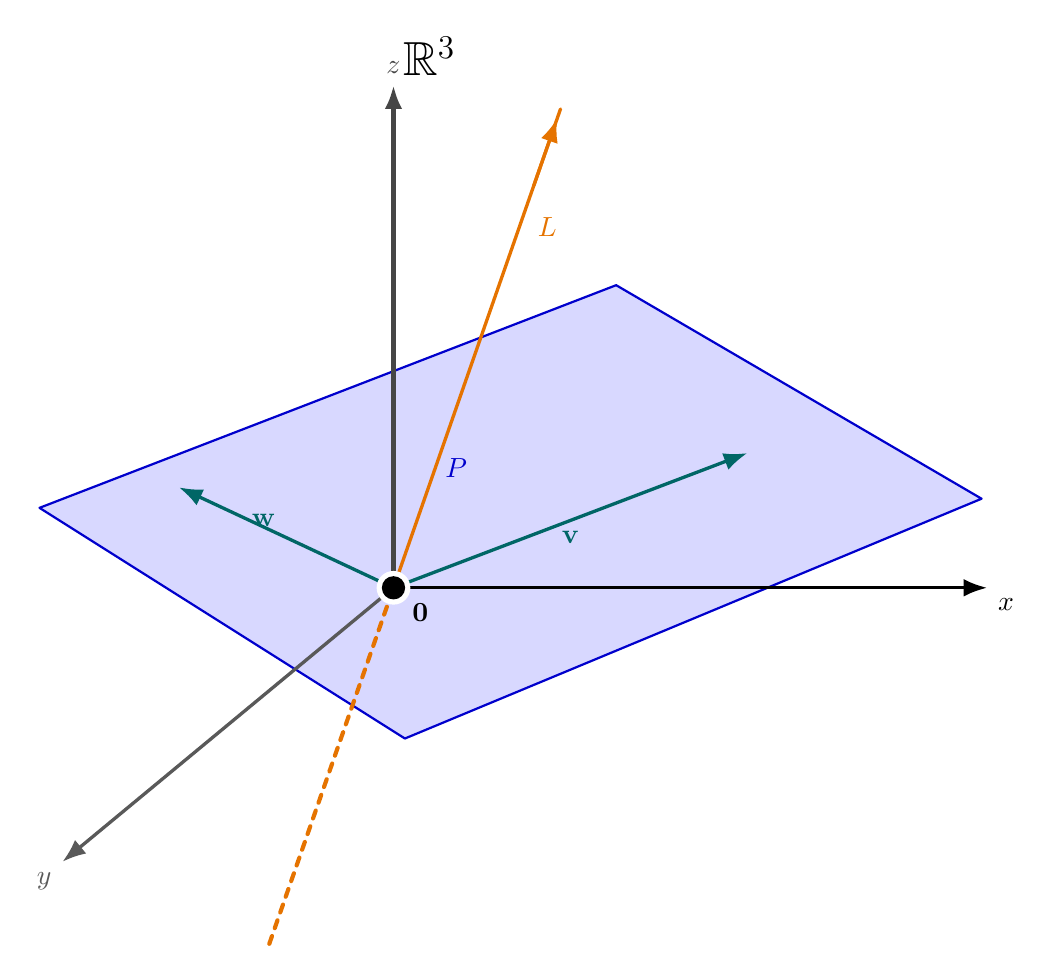
\begin{tikzpicture}[scale=1.45, line cap=round, line join=round]

% --- Colores ---
\colorlet{planecolor}{blue!16}
\colorlet{planeedge}{blue!80!black}
\colorlet{linecolor}{orange!90!black}
\colorlet{veccolor}{teal!80!black}
\colorlet{yaxiscolor}{gray!70!black}
\colorlet{zaxiscolor}{gray!55!black}

% --- Desplazamiento general del sistema ---
\begin{scope}[shift={(0,0.25)}]

% --- Origen y ejes ---
\coordinate (O) at (0,0);
\coordinate (X) at (5.2,0);
\coordinate (Y) at (-2.9,-2.4);
\coordinate (Z) at (0,4.4);

% --- Plano P (paralelogramo) ---
\coordinate (A) at (-3.1,0.70);
\coordinate (B) at (1.95,2.65);
\coordinate (C) at (5.15,0.78);
\coordinate (D) at (0.10,-1.32);

% --- Dirección única de la recta L ---
\coordinate (dir) at (0.75,2.15);

% --- Recta L: misma dirección a ambos lados del origen ---
\coordinate (Lback)  at ($ (O) - 1.45*(dir) $);
\coordinate (Lfront) at ($ (O) + 1.95*(dir) $);

% ===== Dibujo =====

% Plano
\fill[planecolor, opacity=0.95] (A)--(B)--(C)--(D)--cycle;
\draw[planeedge, thick] (A)--(B)--(C)--(D)--cycle;

% Ejes
\draw[-{Latex[length=3mm]}, very thick, black] (O) -- (X) node[below right] {$x$};
\draw[-{Latex[length=3mm]}, very thick, yaxiscolor] (O) -- (Y) node[below left] {$y$};
\draw[-{Latex[length=3mm]}, line width=1.6pt, zaxiscolor] (O) -- (Z) node[above] {$z$};

% Recta L: tramo detrás punteado + tramo delante sólido
\draw[linecolor, dashed, line width=1.5pt] (Lback) -- (O);
\draw[linecolor, very thick] (O) -- (Lfront);

% Flecha solo en el extremo delantero
\draw[-{Latex[length=3mm]}, linecolor, very thick]
  ($(O)!0.84!(Lfront)$) -- ($(O)!0.98!(Lfront)$);

% Vectores en el plano
\draw[-{Latex[length=3mm]}, very thick, veccolor] (O) -- (3.10,1.18)
  node[midway, below] {$\mathbf{v}$};

\draw[-{Latex[length=3mm]}, very thick, veccolor] (O) -- (-1.88,0.88)
  node[midway, above left] {$\mathbf{w}$};

% Origen
\fill[white] (O) circle (4.2pt);
\fill[black] (O) circle (2.9pt);
\node[below right] at (0.08,-0.05) {$\mathbf{0}$};

% Etiquetas
\node[planeedge] at (0.55,1.05) {$P$};
\node[linecolor] at ($(O)!0.73!(Lfront)+(0.28,0.10)$) {$L$};
\node[above right] at (0,4.4) {\LARGE $\mathbb{R}^3$};


\end{scope}

\end{tikzpicture}
\end{document}